\documentclass[conference]{IEEEtran}
\usepackage[T1]{fontenc}
\usepackage{mathptmx}
\usepackage[scaled=0.92]{helvet}
\usepackage{graphicx,booktabs,amsmath,cite,url,xcolor,array,colortbl}
\usepackage[hidelinks]{hyperref}
\usepackage{microtype}
\usepackage{dblfloatfix}
\usepackage{capt-of}
\graphicspath{{figures/}}

% semantic palette shared with the figures (figstyle.py)
\definecolor{ink}{HTML}{1B2A41}
\definecolor{blue}{HTML}{2E5C9E}
\definecolor{teal}{HTML}{1F7F7A}
\definecolor{orange}{HTML}{D9772B}
\definecolor{purple}{HTML}{6B4FA0}
\definecolor{red}{HTML}{B4433A}
\definecolor{gray}{HTML}{8A929B}
\definecolor{band}{HTML}{F3F1EC}
\definecolor{paper}{HTML}{FBFAF7}

\newcommand{\finding}[3]{%
  \begin{minipage}[t]{0.235\textwidth}\raggedright\sffamily
  {\color{gray}\fontsize{15}{15}\selectfont\bfseries #1}\\[1pt]
  {\color{ink}\small\bfseries #2}\\[2pt]
  {\color{ink}\footnotesize #3}
  \end{minipage}}

\begin{document}

\makeatletter
\twocolumn[{%
\begin{center}
{\LARGE\bfseries Five Sensors, One Model: Multimodal Activity Recognition\\[2pt] Under a 100\,MB Constraint\par}
\vspace{5pt}
{\large CUHK-X Challenge 2026, Small Model Track, Team AGX\par}
\vspace{6pt}
{\normalsize Atharv\quad BITS Pilani, K K Birla Goa Campus, India\quad \texttt{atharvgaur591@gmail.com}\par}
\end{center}
\vspace{4pt}
\centerline{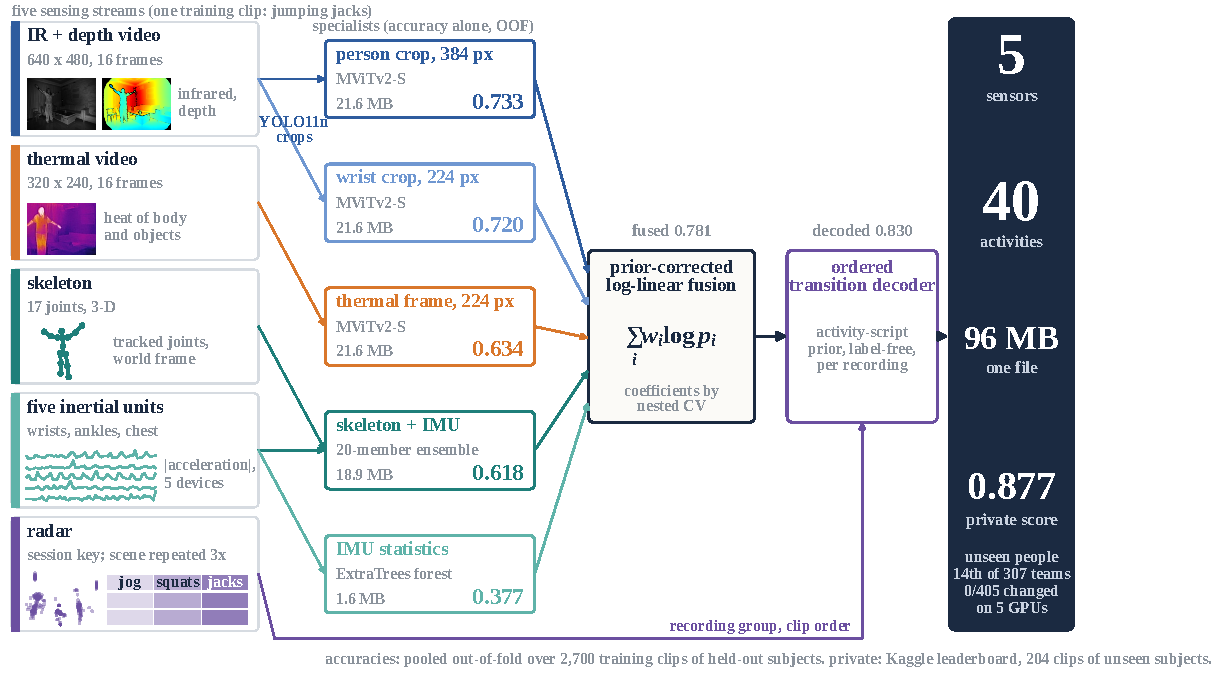
\includegraphics[width=\textwidth]{fig01_abstract.pdf}}
\vspace{2pt}
{\footnotesize Fig.~1.\quad \textbf{Five sensing streams, five specialists, one decision.} One training clip (jumping jacks) seen by every sensor; each specialist reads the stream it is built for; a prior-corrected log-linear fusion combines their posteriors and an ordered transition decoder applies the activity-script structure of a recording session. Member accuracies are pooled out-of-fold over 2,700 training clips from held-out subjects (0.377 to 0.733); the fusion reaches 0.781 and the decoder 0.830. The whole system is one 96.37\,MB file and scored 0.877 on the private leaderboard (14th of 307), with 0 of 405 predictions changing across five GPU generations.\par}
\vspace{5pt}
\begin{minipage}{\textwidth}
\noindent\textbf{\textit{Abstract.}}\quad We classify forty everyday activities from privacy-preserving sensors (infrared and depth video, thermal video, tracked skeletons, five wearable inertial units and radar) for subjects never seen in training, with every inference-time parameter inside one file of at most 100\,MB. The system fuses three small Kinetics-initialised video models that each see a different view (the person crop at 384\,px, the wrist crop at 224\,px, the thermal full frame at 224\,px), a 20-member skeleton/inertial ensemble and an inertial-statistics forest, in a prior-corrected log-linear space with coefficients chosen by nested cross-validation, and decodes each recording group with a label-free activity-script prior. The thesis is that, under this budget and cross-subject shift, accuracy comes from complementary small specialists plus structure rather than from model size: every larger single model we trained lost, and every measured lever that assumed independent evidence failed against the same subject-correlated residual. Four findings shape the design: input resolution helps the body crop and hurts the wrist crop; the thermal camera, useless at 128\,px, becomes a contributing sensor at 224\,px full frame; the five members recover different clips and every one is load-bearing; and fusion raises accuracy on 14 of 16 held-out subjects while narrowing their spread (sd 6.4 to 5.4 points). The frozen 96.37\,MB package scores 0.866 public and 0.877 private, reproduces its submission byte-for-byte in a network-isolated container, loses at most 1.8 points when any single sensor is absent, and is insensitive to its fusion coefficients across a $\pm$50\,\% range.
\end{minipage}
\vspace{5pt}

\noindent\colorbox{band}{\begin{minipage}{\dimexpr\textwidth-2\fboxsep}
\vspace{3pt}
\finding{01}{Resolution is modality-specific}{person crop 0.714 to 0.733 from 224 to 384\,px, flat at 448; wrist crop $-$1.36 points from 224 to 288\,px (Fig.~\ref{fig:res})}\hfill
\finding{02}{Complementary sensors recover different clips}{2,399 of 2,700 clips are right for at least one member, 2,109 for the fusion; removing any member costs 11 to 48 clips (Fig.~\ref{fig:members})}\hfill
\finding{03}{Fusion narrows the subject spread}{16 held-out subjects: mean 73.0 to 78.2, sd 6.4 to 5.4, worst-to-best 23 to 21 points (Fig.~\ref{fig:loso})}\hfill
\finding{04}{Stable under missing sensors and coefficients}{worst single-sensor loss 48 clips of 2,700 ($-$1.8 points); every coefficient $\times$0.5 to $\times$1.5 within $-$24 to $+$7 clips (Fig.~\ref{fig:abl})}
\vspace{3pt}
\end{minipage}}
\vspace{8pt}
}]
\makeatother
\setcounter{figure}{1}

\begin{figure*}[t]\centering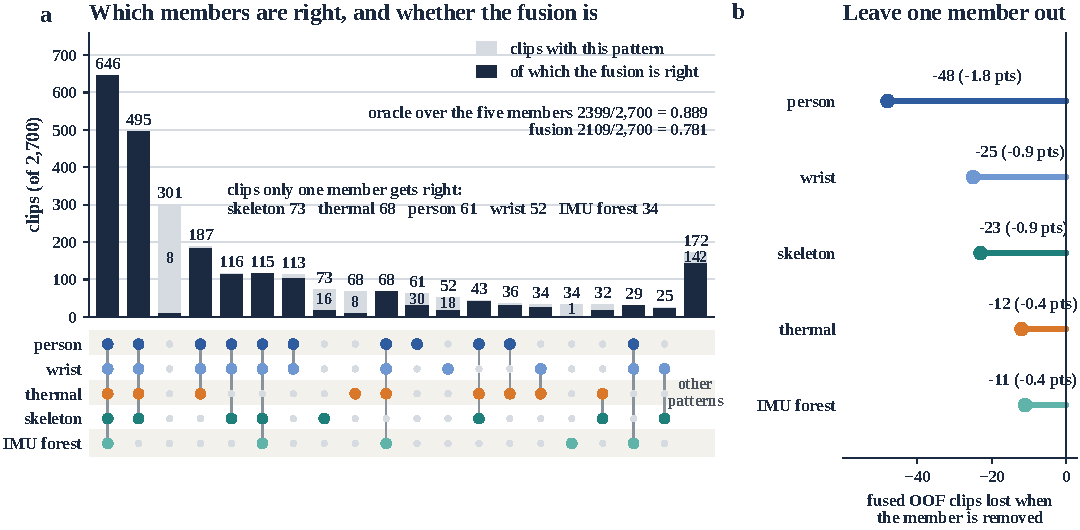
\includegraphics[width=\textwidth]{fig02_complementarity.pdf}
\caption{\textbf{Why five members.} (a)~All 2,700 out-of-fold clips grouped by which members classify them correctly (dots below; patterns with fewer than 25 clips are pooled at the right). Light bars count the clips, dark bars those the fusion gets right. Most clips are easy for everyone (646 all right, 495 all but the forest), 301 are wrong for everyone, and 288 are right for exactly one member: skeleton alone rescues 73, thermal 68, person 61, wrist 52, the forest 34. At least one member is right on 2,399 clips (0.889) against 2,109 for the fusion (0.781): the information is in the members, selection under subject shift is the barrier. (b)~Removing any member from the fusion (weight zero, others fixed) costs 11 to 48 clips; the person view is the most load-bearing.}\label{fig:members}\end{figure*}

\section{Introduction}
Activity recognition from ambient sensors matters most where ordinary cameras are unwelcome: homes, clinics and care settings where identity must not be recorded. The CUHK-X challenge poses the problem in its hard form: 40 fine-grained daily activities, 18 training subjects, evaluation on subjects the model has never seen, a deployable model of at most 100\,MB in a single file, and no test labels of any kind. Under these constraints the useful question is not which single architecture is best, but which \emph{combination of sensing streams and structure} generalises across people while fitting the budget.

Our answer is the thesis of this paper: here, accuracy comes from complementary small specialists plus recording structure rather than from model size. Every larger single model we trained overfit the 2,281-clip training folds (Sec.~\ref{sec:negatives}); five small members, fused in the right probability space and decoded with a prior over activity sequences, beat them, and they do so more uniformly across subjects.

The contributions are measurements rather than claims: (i)~a crop-size rule for video resolution, where higher input resolution pays on the whole-body crop and costs on the already-upsampled wrist crop (Sec.~\ref{sec:resolution}); (ii)~a recipe-transfer result for thermal imaging (Sec.~\ref{sec:thermal}); (iii)~a per-clip account of why five members are needed, and a 16-subject leave-one-subject-out analysis showing that fusion raises 14 subjects and narrows the spread (Secs.~\ref{sec:members}, \ref{sec:subjects}); (iv)~a robustness and reproducibility study of the frozen package (Secs.~\ref{sec:robust}, \ref{sec:repro}); and (v)~a documented set of negative results whose common cause, subject-correlated error, bounds what this family of methods can achieve (Secs.~\ref{sec:negatives}, \ref{sec:limits}).

\section{Task and data}
\noindent\begin{minipage}{\columnwidth}\centering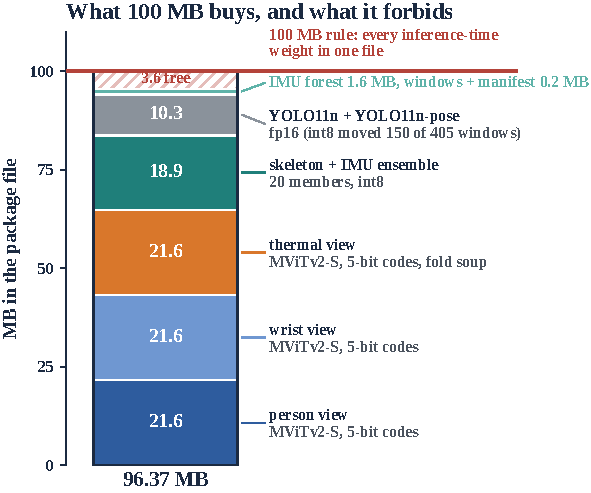
\includegraphics[width=\columnwidth]{fig09_bytes.pdf}
\captionof{figure}{\textbf{The 100\,MB budget as a container.} Compressed bytes of every component in the single package file, from its manifest: three video members at 21.6\,MB each, the skeleton/inertial ensemble 18.9\,MB, both detectors 10.3\,MB, the forest 1.6\,MB, 3.6\,MB free. The budget shaped the architecture: video precision (int5) was chosen to make room for a third view and both detectors, and detector precision was left at fp16 because quantising it changed the inputs.}\label{fig:bytes}\end{minipage}
\vspace{6pt}

The Small Model Track provides 2,933 training clips from 18 subjects and 405 test clips from 4 unseen subjects (201 public, 204 private); an additional held-out set of further subjects is evaluated by the organisers on the frozen package. Each clip holds synchronised infrared and depth frames (640$\times$480), thermal frames (320$\times$240), a 17-joint 3-D skeleton track, recordings from five wearable inertial units (wrists, ankles, chest) and a radar file whose timestamp identifies the recording session (Fig.~1, left). Classes are 40 daily activities, 31 of which involve an object; the training class prior is far from uniform (12 to 335 clips per class, a 28:1 ratio). Recordings are scripted: a subject performs a scene of several activities in a fixed order, and scenes repeat two or three times (Sec.~\ref{sec:decoder}). The metric is top-1 accuracy. Rules verified with the organisers: pretrained standard backbones are permitted; external public data is permitted with declaration (we use none); pseudo-labelling is permitted (the shipped model uses none); all inference-time weights, ensemble members and detectors included, must fit one file of at most 100\,MB.

\section{System}
Fig.~1 is the system. This section gives the parts in the order the data flows.

\subsection{Crops and detectors}
A single square window per clip is taken from a YOLO11n person detection on up to eight infrared probe frames; a second window covers both wrists from YOLO11n-pose keypoints (margin 1.8$\times$, minimum side 96\,px). Infrared and depth are stacked into four channels and sampled at 16 endpoint-uniform frames. When no person is detected the full frame is used (10 of 405 test clips). Both detectors travel inside the package as fp16 tensors and are rebuilt at inference.

\subsection{Video members}
All three video members are torchvision MViTv2-S (34.4\,M parameters) initialised from Kinetics-400, with the patch-embedding stem widened to four channels for the infrared+depth views, trained with one recipe (20 epochs, AdamW, label smoothing 0.1, EMA). The person view runs at 384\,px, the wrist view at 224\,px, the thermal view on the 3-channel full frame at 224\,px; the thermal member is a weight-space average of its four fold models, the person and wrist members are single all-subject models. Horizontal-flip test-time augmentation is applied.

\subsection{Skeleton and inertial ensemble}
Twenty members in five families, four subject-grouped folds each: an adaptive-graph ST-GCN and an ST-GCN on the skeleton, a temporal convolutional network on joint/velocity/bone features, and two temporal convolutional families on the inertial units, one on rotation-invariant features and one in a gravity-aligned world frame (world acceleration, angular velocity, magnitudes, device-presence mask; no absolute orientation, which we found to be a subject/mounting leak). Stored int8, 18.9\,MB.

\subsection{Inertial-statistics forest}
An ExtraTrees classifier (200 trees, depth 12) on 545 per-device statistics, shipped as tensors (1.6\,MB) and evaluated with an exact integer tree walk. Its posterior is Laplace-smoothed: a single exact zero would veto a class for the whole geometric ensemble, a failure we observed before adopting the rule.

\subsection{Fusion in the right prior space}\label{sec:fusion}
Members are combined as $\sum_i w_i \log p_i$. The video members are trained with prior-corrected cross-entropy and emit uniform-prior posteriors; the skeleton ensemble is trained with plain cross-entropy and emits train-prior posteriors, so it is divided by the training prior before fusion. The direction is measured, not assumed: the wrong direction costs four points (0.587 vs 0.627 in an early submission). Coefficients ($w_\text{person}$ 0.236, $w_\text{wrist}$ 0.181, $w_\text{thermal}$ 0.170, $w_\text{skeleton}$ 0.332, $w_\text{IMU}$ 0.297, prior 0.25) are the centroid of the top-25 settings of a nested cross-validation over a 768-point grid, which reproduces the nested-CV estimate without the selection optimism of the argmax.

\subsection{Ordered transition decoder}\label{sec:decoder}
Clips are grouped by their radar session key and ordered by first-frame time; within a group, a first-order transition model over classes, fitted on training metadata only, is applied by beam search with a soft penalty on repeated labels. A clip without a radar key forms its own group and receives the fused argmax. Sec.~\ref{sec:robust} decomposes the decoder's gain and measures what happens when the recording order is not scripted.

\subsection{Fitting 100\,MB}
Fig.~\ref{fig:bytes} shows the budget. The three MViTv2-S members are stored as 5-bit weight codes (symmetric, per output channel, bit-packed), the skeleton ensemble int8, the detectors fp16, the forest as tensors, plus the 405 crop windows of the Kaggle test set (Sec.~\ref{sec:repro}). Int5 costs one public clip against int6 (recovered by the thermal soup); quantising the \emph{detectors} is not free, since int8 moved 150 of 405 crop windows, which is why they stay fp16.


\section{Validation protocol}
Four subject-grouped folds over 16 training subjects give 2,700 pooled out-of-fold (OOF) predictions; fusion coefficients are chosen by nested cross-validation inside them. Eighteen leave-one-subject-out (LOSO) runs per video member and per forest give per-subject accuracies for the shipped ensemble (the skeleton ensemble contributes its 4-fold OOF, which covers 16 subjects and understates it). Adoption of any change required a paired mean gain above two standard errors: the visual seed standard deviation is 1.16 points, so a paired difference carries 1.64, giving a bar of 1.64 on a four-fold mean. OOF accuracy is positively correlated with the public leaderboard ($r=0.91$) but biased high by 8 to 11 points; it was used for screening, never as an adoption criterion on its own. The public split is four subjects: a public score carries $\pm$6.9 clips at one standard error from subject sampling alone. Every figure in this paper is generated by a script from logged artifacts; the numbers plotted and their sources are listed in the figure audit that accompanies the code.


\section{Experiments}
\subsection{What each member contributes}\label{sec:members}
Fig.~\ref{fig:members} answers the question a five-member system must answer first: are the members redundant? They are not. The members disagree on 1,753 of 2,700 clips (every clip that is neither right nor wrong for all five), 288 clips are right for exactly one member, and the single-member rescues are spread across all five, including the weakest (the forest, 0.377 alone, still the only member right on 34 clips). The fusion converts these disagreements well where two or more members agree with the truth (232 of 302 clips with exactly two members right) and poorly where only one does (73 of 288). Leave-one-member-out on the same posteriors (Fig.~\ref{fig:members}b) says every member is load-bearing: person $-$48, wrist $-$25, skeleton $-$23, thermal $-$12, forest $-$11 clips. The oracle over the five members reaches 0.889; what separates it from the fusion's 0.781 is selection, and Sec.~\ref{sec:negatives} reports that every attempt to learn that selection from posteriors failed.

\subsection{Resolution and the crop-size rule}\label{sec:resolution}
\begin{figure}[t]\centering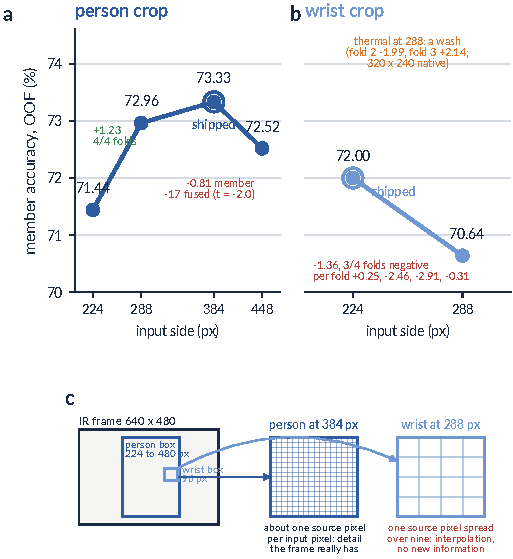
\includegraphics[width=\columnwidth]{fig03_resolution.pdf}
\caption{\textbf{Resolution helps the body crop and hurts the wrist crop.} (a)~Person view: 0.7144, 0.7296, 0.7333, 0.7252 at 224, 288, 384, 448\,px (pooled member OOF); 224 to 288 is positive on 4 of 4 folds, 448 is negative on the member ($-$0.81) and in fusion ($-$17 clips, $t=-2.0$). (b)~Wrist view: $-$1.36 points from 224 to 288\,px, negative on 3 of 4 folds; thermal at 288 is a wash. (c)~The mechanism: a person box spans 224 to 480 source pixels, so a 384-px input samples detail the frame really has; a wrist box is about 96 source pixels, so a 288-px input spreads each source pixel over nine and adds interpolation, not information.}\label{fig:res}\end{figure}
Resolution pays where the crop is large relative to the source frame and costs where the crop is already upsampled (Fig.~\ref{fig:res}). The rule was stated before the wrist experiment was run and was confirmed by it; it also predicted the flat step from 384 to 448\,px, where the person box itself is at the frame's resolution. The practical consequence is where not to spend GPU hours: no higher resolution for the wrist or thermal views.

\subsection{Thermal at full frame}\label{sec:thermal}
\begin{figure}[t]\centering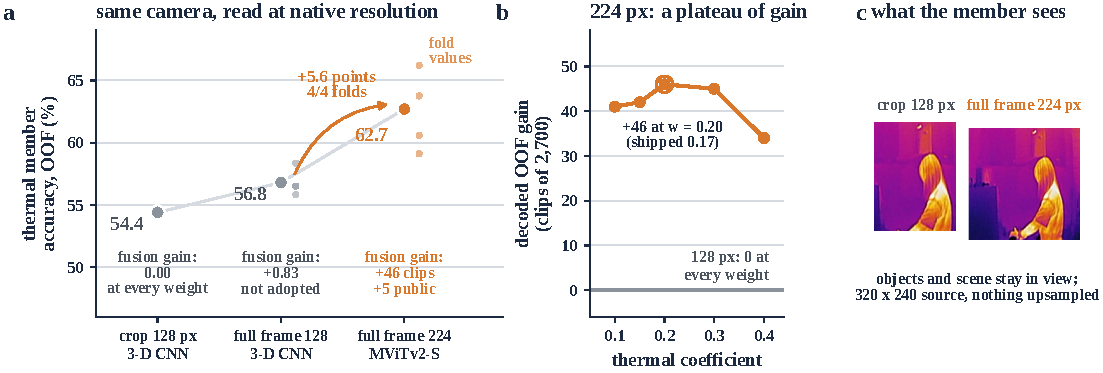
\includegraphics[width=\columnwidth]{fig04_thermal.pdf}
\caption{\textbf{The same thermal camera, read differently.} (a)~Member accuracy of the thermal view at three processing stages: a 128-px person crop through a 3-D CNN (0.544; zero contribution in fusion at every weight from 0.05 to 0.35), the 128-px full frame through the same CNN (0.568; $+$0.83 in fusion, below the bar), and the 224-px full frame through the MViTv2-S recipe (0.627, $+$5.6 points on 4 of 4 folds, small dots). (b)~With the 224-px member, fusion gains 41 to 46 decoded OOF clips across a three-fold range of coefficient, and 5 public clips; at 128\,px the gain is zero at every weight. (c)~What the member sees: the 320$\times$240 source is read near-natively and the objects and scene stay in view. The sensor did not change; the reading of it did.}\label{fig:thermal}\end{figure}
Thermal imaging is the dataset paper's strongest single sensor, yet our 128-px cropped thermal member scored 0.544 and contributed nothing in fusion at any coefficient (Fig.~\ref{fig:thermal}). Applying the video recipe at 224\,px on the full frame raised the member to 0.627 pooled OOF and, for the first time, made it positive in fusion: $+$46 of 2,700 clips through the decoder and $+$5 public clips (167 to 172). The mechanism the figure shows is the crop-size rule again from the other side: thermal frames are 320$\times$240, so 224\,px is near native and nothing is upsampled, and the full frame keeps the objects and the station that the 40 classes are largely defined by.

\subsection{Subject-level generalisation}\label{sec:subjects}
\begin{figure}[t]\centering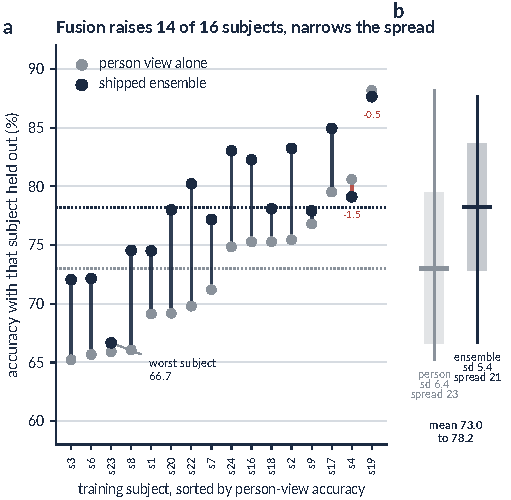
\includegraphics[width=\columnwidth]{fig05_subjects.pdf}
\caption{\textbf{Fusion raises subjects and makes them more alike.} (a)~Leave-one-subject-out accuracy of the person view alone (gray) and of the shipped ensemble (dark) for the 16 training subjects covered by both, each subject a vertical pair sorted by the person-view value; 14 pairs go up, two go down by 0.5 and 1.5 points. (b)~The same values as distributions (mean, $\pm$1 sd box, range): mean 73.0 to 78.2, sd 6.4 to 5.4, worst-to-best spread 23 to 21 points. Over all 18 subjects the person view has sd 6.9 and spread 28 (two subjects lack an ensemble value). The private and held-out stages are draws of unseen subjects, so the narrower spread is the property that matters there.}\label{fig:loso}\end{figure}
Fig.~\ref{fig:loso} reports the 16-subject paired comparison. The shipped ensemble beats the person view alone on 14 of 16 held-out subjects, by $+$5.2 points on average, with the two exceptions within seed noise (user4 $-$1.5, user19 $-$0.5). The dispersion falls as well: the standard error of an 8-subject draw, which is what the private and held-out evaluations are, drops from 2.4 to 1.9 points. A lower-quartile selection statistic that re-ranks subjects per configuration turned out to reward shuffling (it compares different subject sets); we replaced it with a fixed worst-four set and the paired per-subject delta, which is what the figure reports.

\subsection{Robustness of the frozen system}\label{sec:robust}
\begin{figure}[t]\centering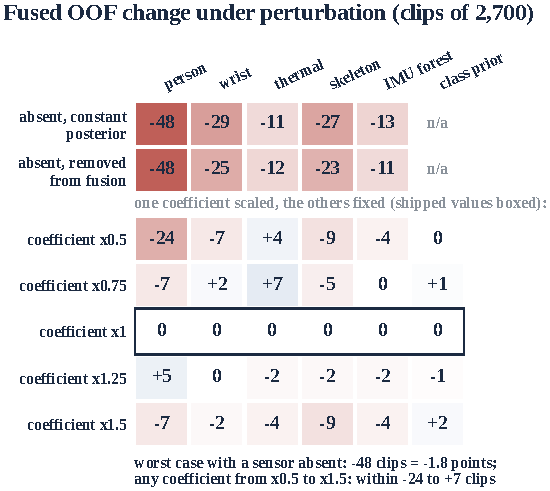
\includegraphics[width=\columnwidth]{fig06_robustness.pdf}
\caption{\textbf{Stability atlas of the frozen fusion.} Change in fused OOF accuracy (clips of 2,700, pre-decoder, baseline 2,109) when (a)~one sensor is absent, either replaced by the member's constant posterior, as the pipeline does for a missing modality, or removed from the fusion; and (b)~one fusion coefficient is scaled by 0.5 to 1.5 with the others fixed. Worst single-sensor loss 48 clips (1.8 points); every coefficient cell within $-$24 to $+$7 clips. The shipped centroid sits on a plateau, which is also why any re-weighting moves at most 8 of the 405 test rows.}\label{fig:abl}\end{figure}
\begin{figure*}[t]\centering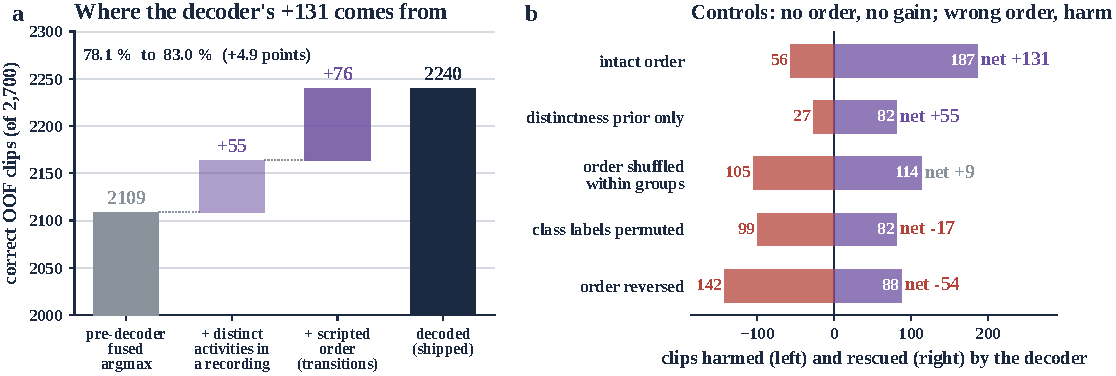
\includegraphics[width=\textwidth]{fig07_decoder.pdf}
\caption{\textbf{Where the decoder's gain comes from, and when it disappears.} (a)~Decoded OOF accuracy built up from the pre-decoder fused argmax (2,109): the label-free ``distinct activities within a recording group'' prior alone gives $+$55 (transition model replaced by uniform), the scripted order on top of it $+$76, together $+$131 (2,240, 83.0\,\%). (b)~Rescued and harmed clips under controls: intact order 187/56; distinctness prior only 82/27; clip order shuffled within groups 114/105 (net $+$9); class labels permuted in the transition model 82/99 (net $-$17); order reversed 88/142 (net $-$54). Without recording structure the decoder is neutral; only a systematically wrong order harms.}\label{fig:dec}\end{figure*}
\emph{Missing sensors} (Fig.~\ref{fig:abl}a): no single absent sensor costs more than 48 clips of 2,700 (1.8 points); the person view is the most load-bearing, thermal and the forest the least. Absent modalities are handled deterministically as zero inputs, exactly as in the Kaggle run, where 10 clips have no thermal frames. \emph{Coefficients} (Fig.~\ref{fig:abl}b): every setting within $\pm$50\,\% of the shipped values lies within $\pm$1\,\% of the baseline. \emph{Recording order} (Fig.~\ref{fig:dec}): about half of the decoder's gain comes from the distinctness prior ($+$55) and half from the scripted order ($+$76); if a recording does not follow the script the decoder is neutral ($+$9), and only a systematically reversed order harms. Permuting the class labels inside the transition model removes the gain ($-$17), so the decoder is not memorising label frequencies.

\section{Negative results}\label{sec:negatives}
\begin{figure*}[t]\centering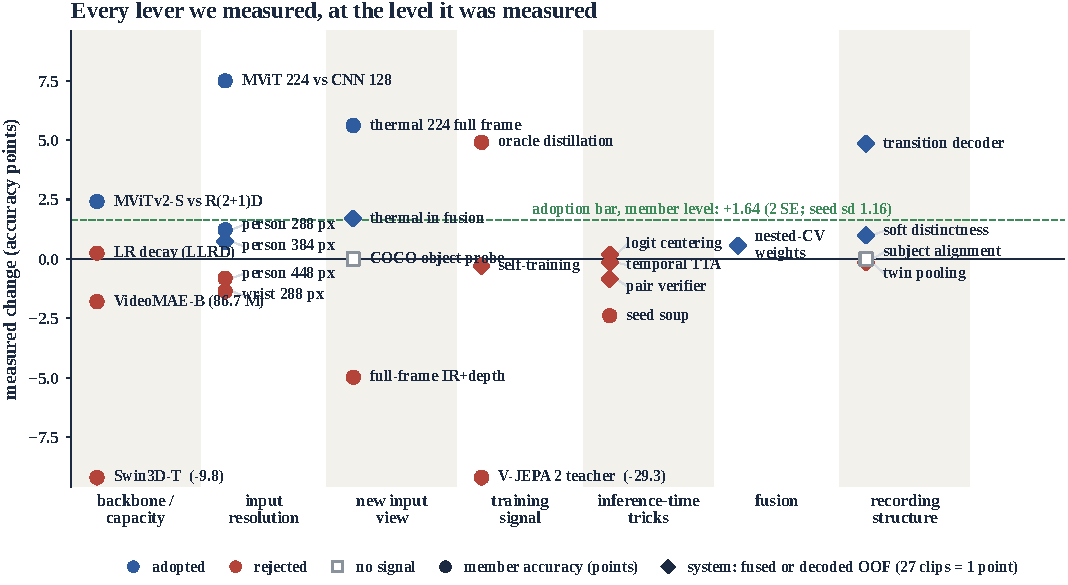
\includegraphics[width=\textwidth]{fig08_landscape.pdf}
\caption{\textbf{The experiment landscape.} Every lever measured during the campaign, placed in the lane of what it changed and at the level it was measured: member accuracy in points (circles) or the fused/decoded OOF system in points (diamonds, 27 clips = 1 point); hollow squares are probes with no signal (AUC 0.50, cluster purity 0.34). Blue was adopted, red rejected, in each case by the paired-fold rule; the dashed line is the member-level adoption bar. Two rejected levers are off scale (Swin3D-T $-$9.8, a frozen V-JEPA~2 teacher $-$29.3). Capacity, training signal and inference-time tricks cluster at or below zero; the adopted levers are resolution, a new input view read correctly, prior-space fusion and recording structure.}\label{fig:landscape}\end{figure*}
We tested the obvious routes to more accuracy and Fig.~\ref{fig:landscape} places each result. Larger or different backbones lost: VideoMAE-B ($-$1.80, 0 of 4 folds; 86.7\,M parameters fine-tuned on 2,281 clips), Swin3D-T ($-$9.8, a 32-frame model fed 16 frames). A frozen video foundation model as a teacher was 29 points behind our own member (V-JEPA~2 ViT-L 0.419 vs 0.712). Distillation from our own oracle targets improved a member by $+$4.9 on one fold but the student alone scored 157 public and the fused pair 165 against the 167 champion. Recipe changes were null (layer-wise LR decay $+$0.25, sd 1.79). Full-frame infrared+depth was a correlated copy of the person crop ($-$5.0 on the member, $+$8 clips at best in fusion). A COCO detector could not name the object in the hand (AUC 0.50 against 0.57 for the station alone). Inference-time tricks bought member accuracy with diversity and lost it in fusion: temporal test-time augmentation ($+$0.5/$+$0.9 on the members, $-$4 clips fused), seed soups ($-$2.39, 4 of 4 folds), a pair verifier on trunk features ($-$0.84 on the decidable clips). Transductive self-training raised the member $+$1.38 and lowered the fusion, because pseudo-labels from the fusion pull the member toward it. Twin pooling across repeated scenes was $+$1 before and $-$4 after the decoder.

The common cause is measured (Sec.~\ref{sec:limits}): the residual error is per-subject and correlated, and each lever above assumes independent evidence. The negatives are the map of where the bottleneck is not: it is not capacity, not the training recipe, and not per-clip arbitration.

\section{Reproducibility and efficiency}\label{sec:repro}
\begin{figure}[t]\centering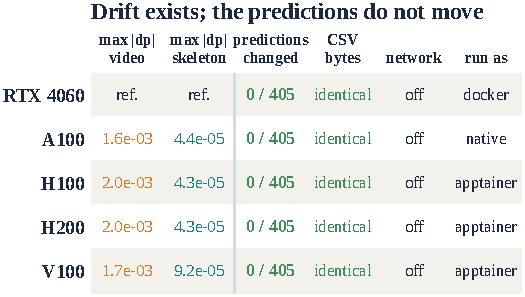
\includegraphics[width=\columnwidth]{fig10_verification.pdf}
\caption{\textbf{Verification matrix.} The frozen package run on five GPU generations, three of them from the shipped container image. Posterior differences against the reference run exist (up to $2\times10^{-3}$ for the video members, $10^{-4}$ for the skeleton ensemble, none for the forest); the fused prediction changes on 0 of 405 clips on every generation and the CSV is identical. The claim is unchanged predictions, not bit-level equality.}\label{fig:gpu}\end{figure}

\begin{table}[t]
\caption{Result card of the frozen submission.}\label{tab:card}
\centering\footnotesize
\begin{tabular}{@{}l>{\raggedright}p{1.55cm}p{4.0cm}@{}}
\toprule
\textbf{metric} & \textbf{result} & \textbf{interpretation} \\
\midrule
private accuracy & \textbf{0.877} & 179/204, 14th of 307 teams \\
public accuracy & 0.866 & 174/201, four subjects \\
package size & \textbf{96.37\,MB} & one file, under the 100\,MB rule \\
inference & 0.39\,s/clip & A100, 405 clips in 2\,min\,39\,s \\
 & 0.72\,s/clip & RTX 4060 laptop, peak GPU memory 5.4\,GB \\
prediction drift & \textbf{0/405} & five GPU generations, network off \\
reproduction & byte-identical & second selected submission \\
 & 403/405 & primary submission, two disclosed near-ties \\
\bottomrule
\end{tabular}
\end{table}

One command, \texttt{bash inference.sh <data\_dir> <out.csv>}, regenerates the submission from raw frames: detectors extracted from the package, caches rebuilt, members reconstructed from tensors, fusion with the declared coefficients, decoder. It runs without network access (models are built without pretrained weights and loaded from the package; an empty \texttt{TORCH\_HOME} would make any download attempt fail) and never writes under the data directory. Fig.~\ref{fig:gpu} characterises five GPU generations against the laptop run that produced the submitted file; Table~\ref{tab:card} collects the outcomes. The only member-level argmax change anywhere is the thermal member on one clip, absorbed by the fusion. Crop-window computation by the detector does drift across GPUs (recomputing on another GPU changed 22 of 405 rows), so the Kaggle windows travel inside the package, gated by a fingerprint of the clip's frame filenames; any other clip is detected live. A hostile synthetic test set (reused clip ids on different recordings, new id schemes, missing radar, thermal, skeleton, inertial or infrared data, 320$\times$240 frames, zero-byte files, stray folders, shuffled or absent submission templates) runs to completion with the rows in the requested order. The package was verified from the actual upload archives in a clean directory with the working repository removed, twice.

One disclosed residual: the primary selected submission was fused from the skeleton ensemble's full 48-member output before that ensemble was pruned to fit the budget; the package reproduces it in 403 of 405 rows (two decoder near-ties, margins 0.012 and 0.006), and an exhaustive search over about 900 coefficient settings with the frozen tensors comes no closer than one row. We ship the principled coefficients and document the two rows rather than fit to the target file.

\section{Limitations}\label{sec:limits}
\begin{figure}[t]\centering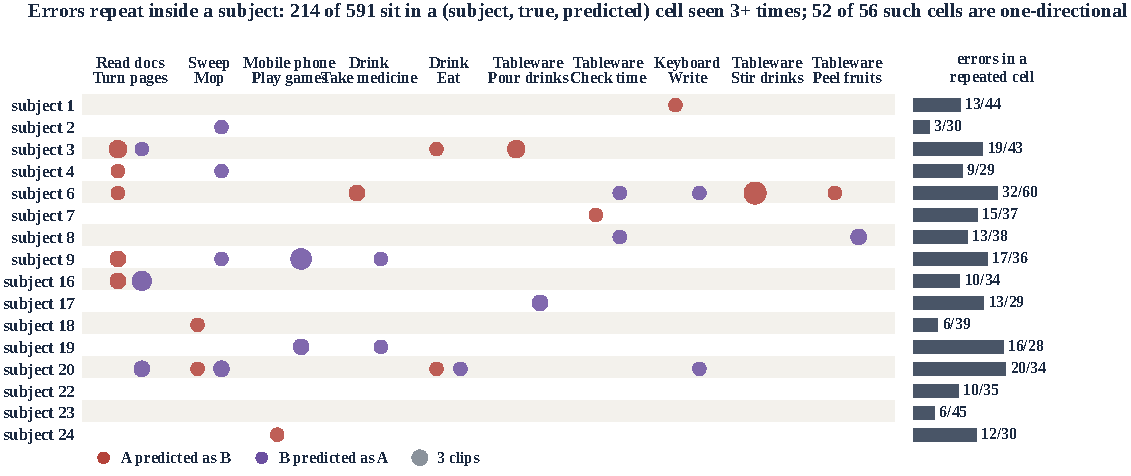
\includegraphics[width=\columnwidth]{fig11_errors.pdf}
\caption{\textbf{The residual error is subject-correlated.} Shipped fusion on the 2,700 OOF clips: 214 of 591 errors sit in a (subject, true class, predicted class) cell that occurs three or more times, and 52 of the 56 subject-level class-pair cells are one-directional (a subject who reads documents is called turning pages every time, never the reverse). Dot area is the number of clips; the right bars give each subject's share of errors in repeated cells. The same statistic on the earlier champion fusion was 229 of 658 (EXP-132).}\label{fig:errors}\end{figure}
Public accuracy is 0.866 against a leaderboard top of 0.985: the members are information-rich (oracle 0.889) and the barrier is selection under subject shift, which no per-clip lever we tested moves. Fig.~\ref{fig:errors} shows why: errors are not independent mistakes on hard clips but subject-constant offsets (twin recordings share the identical wrong label 68\,\% of the time), and a subject-constant offset is invisible to any per-clip model by construction. The skeleton ensemble's pruning step was not logged at the time (its tensors are hashed and shipped verbatim; the recipe of every member is recorded). The decoder's gain depends on scripted recordings; it is neutral, not harmful, when the script is absent.

\noindent\colorbox{band}{\begin{minipage}{\dimexpr\columnwidth-2\fboxsep}\vspace{3pt}\sffamily\footnotesize
\textbf{\color{red}More model}: measured, no gain. Larger backbones, a foundation teacher, distillation, soups, test-time augmentation and 448\,px all failed the paired-fold bar (Fig.~\ref{fig:landscape}).\\[3pt]
\textbf{\color{blue}More subjects}: the direction the evidence points to, not a quantified prediction. The residual is per-subject (Fig.~\ref{fig:errors}); a linear probe on frozen features saturates by six subjects (EXP-136), so any gain would have to come through the representation, which we have not measured.
\vspace{3pt}\end{minipage}}

\section{Conclusion}
Under a 100\,MB budget and cross-subject evaluation, five small sensing specialists, fused in the right probability space and decoded with the structure of the recording, beat every larger single model we trained and generalise more evenly across people. The design rests on measured rules (resolution is modality-specific; a sensor's value depends on how it is read; every member is load-bearing; the fusion is on a plateau) and its limits are measured too: the remaining error is subject-correlated, and more capacity is not the next lever.

\section*{Declarations}
Pretrained weights: torchvision MViTv2-S (Kinetics-400); Ultralytics YOLO11n and YOLO11n-pose (COCO). No external datasets, no test labels, no leaderboard probing, no pseudo-labels in the shipped model. All code, the experiment log (EXP ids cited in the figure audit), the figure scripts and the package are in the repository at tag \texttt{verification-v1}.

\end{document}
